\chapter{Implementation}

\section{Overview}

This chapter describes the changes and enhancements that were made to
Elektra in order to answer the research questions.
First we talk about Elektra's plugin API in general and how we used it
to introduce cryptographic operations to Elektra. Then the concept of
the key management is presented. At last some interesting implementation
details about the crypto libraries used are given.

\section{Elektra Components}\label{elektra-plugins}

\subsection{Key and Keyset}

Elektra abstracts configuration parameters in a hierarchical key-value database.
A keyset holds zero or more keys.
The key holds its path within the configuration hierarchy as well as the configuration parameter either as a string value or as a binary value.
A key may also contain meta-keys, which are keys that further describe the key.
Elektra uses meta-keys for different purposes:

\begin{enumerate}
\item state information of the key (e.g. encrypted, encoded, ...)
\item data validation (for example: numeric value, binary value, ...)
\item formatting (for example: position in file, number of spaces/tabs between parameters, ...)
\end{enumerate}

\subsection{Plugin}

The core of Elektra is kept small, meaning that it provides mainly the database abstraction as well as a plugin system.
All the configuration access operations (mainly file reads and writes but there are more complicated constructs, like intercepting \texttt{open()} calls in order to inject a Mozilla configuration, as well) are performed by plugins.
The plugins should fulfill exactly one purpose, keeping to the UNIX philosophy.
To give an example: one plugin may write to \texttt{/etc/hosts} and another one may encode binary values using the Base64 encoding scheme.

A plugin can export different methods in order to fulfill its purpose.
They are enumerated below:

\subsubsection{checkconf}\label{checkconf}

At this method a plugin may validate the backend configuration as well as
the plugin configuration. The plugin may modify the configuration or
report that the configuration is incomplete or wrong in some way.

\subsubsection{open}\label{open}

The \texttt{open} method is called to initialize the plugin.

\subsubsection{close}\label{close}

The \texttt{close} method is called to properly shutdown the plugin and
release all resources it may hold.

\subsubsection{set}\label{set}

For storage plugins the \texttt{set} method is called when changes made to the key-value
database should be persisted.
Filter plugins export this method to modify the keyset (for example: encode binary values using the Base64 schema).

\subsubsection{get}\label{get}

The \texttt{get} method is called when the content of the key-value
database is requested by an application.
Filter plugins provide this method to transform data in the keyset (for example: decoding Base64 encoded strings back into their corresponding binary value).
Storage plugins typically perform read operations within this method.

\subsection{Backend}

Backends are one or more plugins combined into a unit that interact with a single configuration point (typically a configuration file).
The backend is ''mounted`` into Elektra's configuration hierachy.
This process is similar to the mounting process in UNIX-like file systems, where a device can be mounted to a specific directory in the virtual file system.
In terms of Elektra the virtual file system is the key-value database and the device is the configuration file.
Every backend has its own configuration itself (i.e. backend configuration), which specifies the runtime behavior of the plugins within the backend.

\subsection{Compilation Variants}

Elektra's build scripts provide a functionality called compilation variants, which means a plugin is being compiled multiple times with minor differences.
This is useful if a feature (for example: cryptographic operations) is provided by different libraries interchangeably.
A lot of the plugin code stays the same for every compilation variant except for the library-specific calls.
Those calls are encapsulated using C preprocessor directives.
The following code snippet further illustrates the usage of compilation variants:

\begin{lstlisting}[language=C,caption={Example usage of compilation variants in Elektra}]
static int elektraCryptoInit (Key * errorKey)
{
#if defined(ELEKTRA_CRYPTO_API_GCRYPT)
	return elektraCryptoGcryInit (errorKey);
#elif defined(ELEKTRA_CRYPTO_API_OPENSSL)
	return elektraCryptoOpenSSLInit (errorKey);
#elif defined(ELEKTRA_CRYPTO_API_BOTAN)
	return elektraCryptoBotanInit (errorKey);
#else
	return 1;
#endif
}
\end{lstlisting}

As we can see every crypto library is handled differently but the code frame of the plugin stays the same for all compilation variants.

\section{Crypto Plugin}\label{crypto-plugin}

\subsection{Reasons For Developing The Plugin}

In order to evaluate our performance related questions we need a reference application with a high degree of modularity.
The modularity is required to gain profound insight in the runtime behavior of the reference application.
By combining different modules (or plugins) or disabling certain modules we can test a variety of possible use cases.

Elektra provides the required degree of modularity but it did not provide any cryptographic functions when we started working on this thesis.
So we choose to develop a crypto plugin for Elektra, that enables us to use Elektra as benchmark environment.

\subsection{Benefits for the Elektra Project}

Elektra is a configuration database and as such it will be used for storing sensitive configuration data (for example: database passwords) at some point.
Leaving this information unencrypted is a security threat.
The \crypto{} is a way of tackling this issue by providing transparent encryption.
This means that the information is stored encrypted on the filesystem and is decrypted by Elektra whenever the application requests its configuration (thus the encryption/decryption works transparent to the user). The \crypto{} can simply be added to a backend and thus integrates well with other Elektra plugins.

\subsection{Challenges}

The first challenge was to design a single plugin or several plugins that support different providers for cryptographic operations.
With the goal of comparability in mind, the plugin architectures must be very similar for each crypto-provider.
Otherwise no useful conclusions can be drawn from differing benchmark results.
Finally we decided to implement one single crypto plugin that handles the encryption and decryption of keysets.
Elektra's compilation variants enabled this architecture.
For every crypto-provider or crypto library we want to integrate, a new compilation variant is added to the plugin.

The next problem was how to create, generate, derive or restore the keys for the cryptographic operations.
This part of the plugin is crucial from a security perspective.
Any kind of wrongdoing in this module could lead to leaks, endangering the confidentiality of the protected data.
The first design that came to mind was a password based schema that utilizes the Password-Based Key Derivation Function 2 (PBKDF2).\footnote{PBKDF2 is specified in RFC 2898.}
However this approach was not suitable for any kind of batch operation as the program flow would interrupt and ask for password input.
So we decided to delegate the handling of cryptographic keys to an existing key store: GnuPG.
GnuPG in combination with the pinentry utilities turned out to be a great way of managing keys.
In addition the users benefit from this approach because they can simply use their existing PGP keys for securing their data in Elektra.

In the following section we are going to dive deeper into the technical
details of the implementation of the \crypto.

\subsection{Technical Aspects}

The \crypto{} acts as a filter that is applied to the keyset before the storage plugin reaches its \texttt{kdb set} phase.
In Elektra terms this stage is called \texttt{presetstorage}.
Later on when the encrypted data is requested the plugin decrypts the keyset after the storage plugin read the configuration in its \texttt{kdb get} phase.
This stage is called \texttt{postgetstorage} in Elektra.

Not all keys in the keyset are considered for encryption or decryption.
The \crypto{} uses a metakey to identify which keys have to be processed.
If a metakey with name \texttt{``crypto/encrypt''} is set to a value of \texttt{``1''} then the key is marked for encryption.
During \texttt{presetstorage} the plugin checks the metakey and only encrypts values if the metakey is set properly.
Decryption in the \texttt{postgetstorage} phase works analogous.
All other keys, which are not marked, are ignored and left unchanged by the plugin.

In the following section we explain how the encryption and decryption process works in detail.

\subsection{Cryptographic Details}

\subsubsection{Data Types}

\paragraph{elektraCryptoHandle} is a structure that  abstracts the crypto
library specific data types which hold cryptographic keys and initialization
data for the cryptographic processes (for example: initialization vectors).

Other than the handle, the \crypto{} does not require any further
special data types.

\subsubsection{Message Structure}

The \crypto{} operates on Elektra's key data type. During its work it modifies
the value as well as the meta-data of the keys. The value is always
transformed into binary data. In order to restore the value to its original
type during decryption, some header information has to be stored.

The following information is encoded into the first cryptographic block during
encryption:

\begin{table}[h!]
\centering
\caption{Structure of the crypto message header}
\label{my-label}
\begin{tabular}{clrrl}
	\textbf{} & \textbf{element}                          & \textbf{offset} & \textbf{length} & \textbf{data type}    \\ \hline
	$L_S$     & length of the salt                        & 0               & 4 B             & unsigned long integer \\
	$S$       & salt                                      & 4               & $L_S$ B         & byte                  \\
	$T$       & original data type (string, binary, null) & 4 + $L_S$       & 1 B             & byte (flag)           \\
	$L_C$     & original content length                   & 5 + $L_S$       & 4 B             & unsigned long integer \\ \hline
\end{tabular}
\end{table}

The salt is a sequence of random bytes and is used in cryptography to prevent
table-based key guessing attacks.
The content length is saved because most crypto libraries do not support
padding out of the box, which means that they always operate on whole blocks
of data, where the block size depends on the cryptographic algorithm that is
used.

\subsubsection{Methods}

\paragraph*{open}

\paragraph*{get}
see figure \ref{impl_decrypt} on page \pageref{impl_decrypt}...

\begin{figure}[h]
\center
\caption{Decryption of a keyset at the kdb get method}
\label{impl_decrypt}
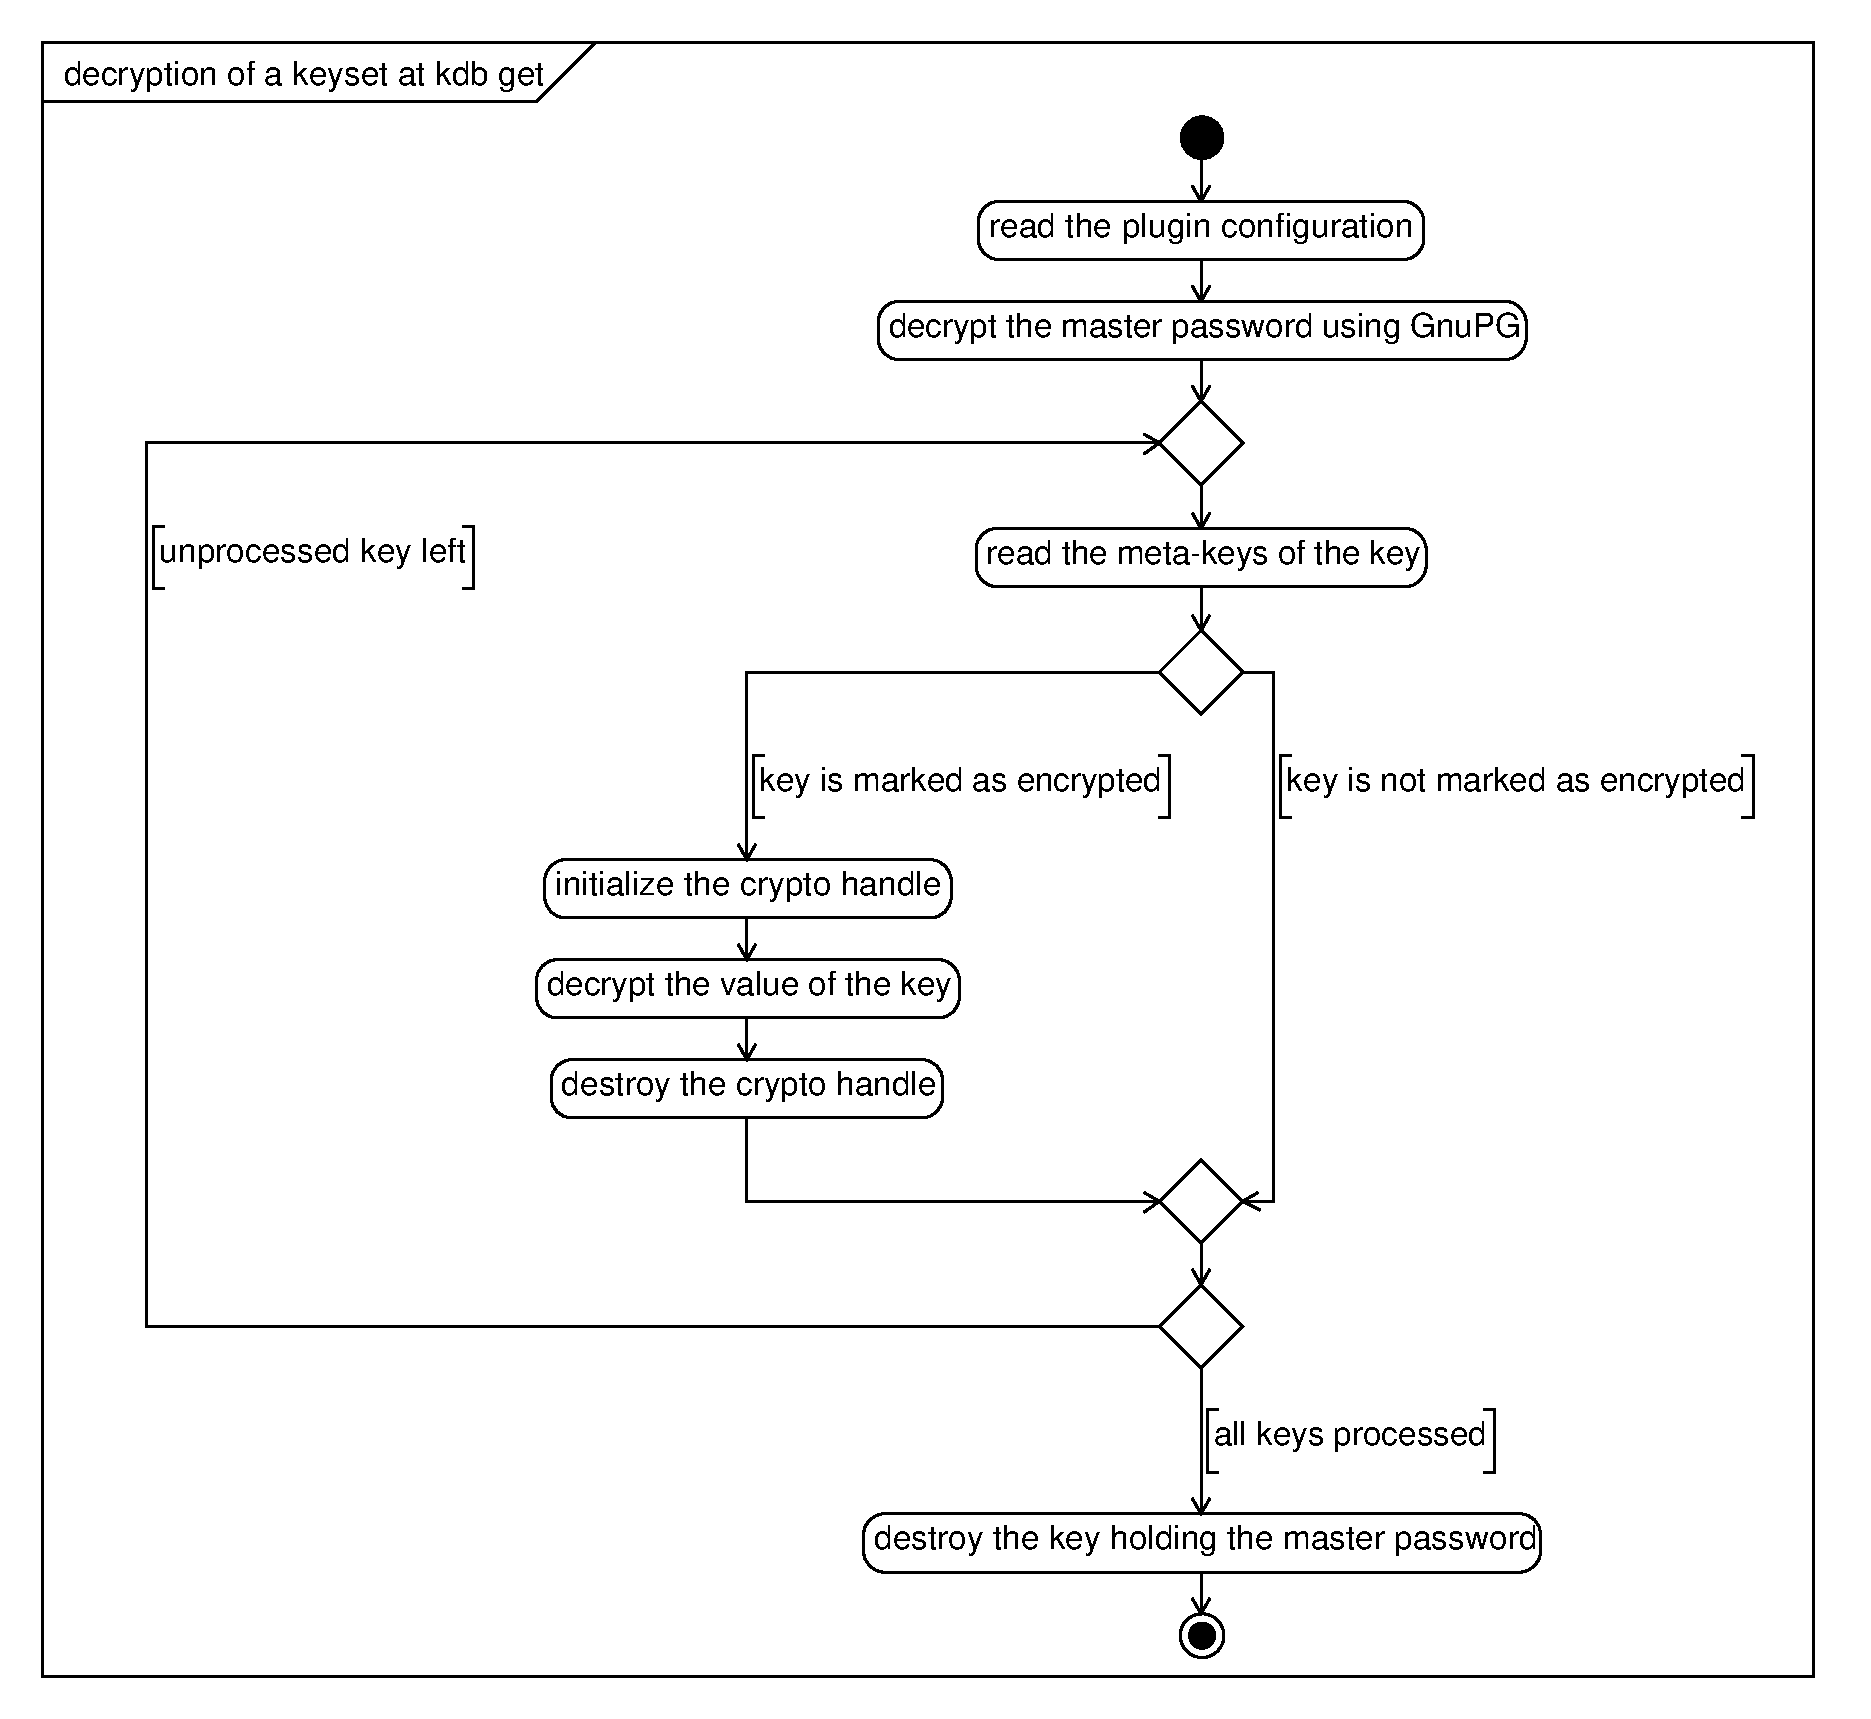
\includegraphics[width=15.0cm]{umlet-figures/impl_decrypt.pdf}
\end{figure}


\paragraph*{set}
see figure \ref{impl_encrypt} on page \pageref{impl_encrypt}...

\begin{figure}[h]
\center
\caption{Encryption of a keyset at the kdb set method}
\label{impl_encrypt}
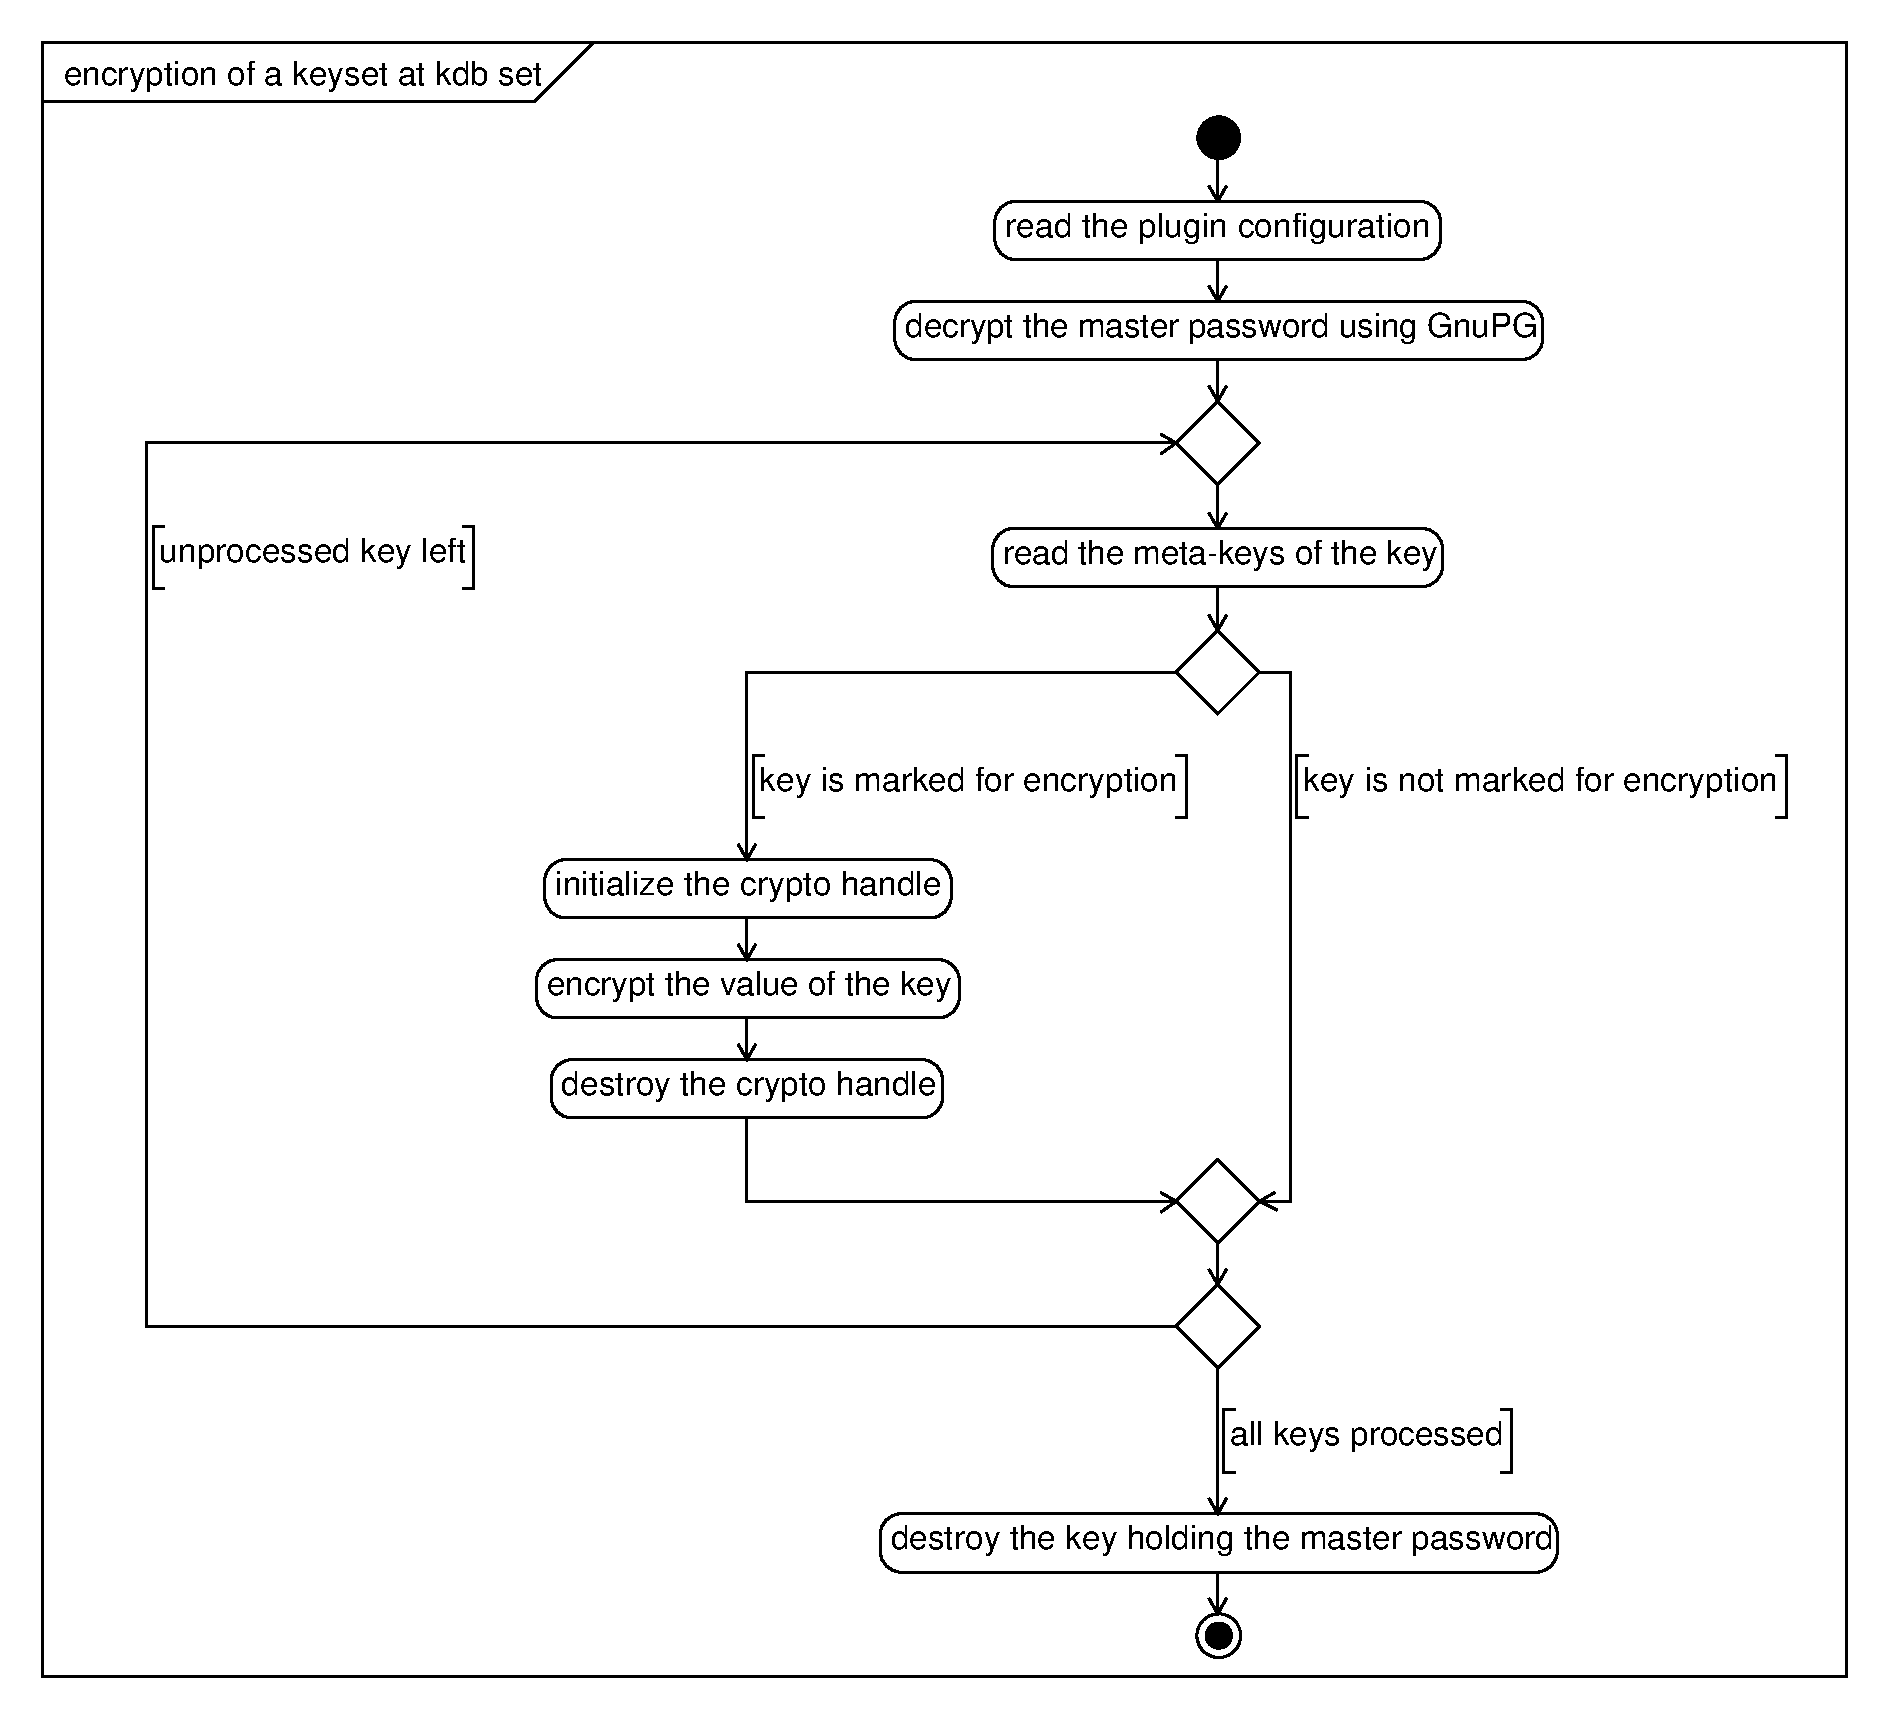
\includegraphics[width=15.0cm]{umlet-figures/impl_encrypt.pdf}
\end{figure}


\paragraph*{close}


\subsubsection{Compilation Variants}


\subsubsection{Key Management}



\subsection{Details About The Crypto Libraries}\label{details-about-the-crypto-libraries}



\section{Fcrypt Plugin}\label{fcrypt-plugin}

\subsection{Reasons For Developing The Plugin}

% crypto not good for entire config files -> too much overhead
% other performance benchmark -> GPG also uses libgcrypt

\subsection{Benefits for the Elektra Project}

% Users can encrypt entire configuration files
% no compile-time dependency which is nice for developers

\subsection{Challenges}

% Elektras internal API -> sync plugin workaround

\subsection{Technical Aspects}

% cryptographic operations are entirely handled by GnuPG


The \fcrypt{} was written to encrypt and decrypt whole files using the GPG interface mentioned before.
One of its advantages is that there are no dependencies at compile time.
Only the \texttt{gpg2} or \texttt{gpg} binary are required as runtime dependency.

Again the GPG keys to be used for encryption are defined in the plugin configuration following the same semantics as the \crypto{}.

% Chapter Outro

This chapter explained the Elektra plugin system and how we used it to introduce cryptographic methods to the Elektra project.
Now that we have an application to examine, we continue with the description of the actual measurements in the following chapter.
